\documentclass[a4paper,12pt]{book}
\usepackage[utf8]{inputenc}
\usepackage{hyperref}
\usepackage{graphicx}
\usepackage{amsmath}% http://ctan.org/pkg/amsmath
\usepackage{amsthm}
\newtheorem{thm}{Theorem}[chapter]
\newtheorem{example}[thm]{Example}
\begin{document}

\author{Kevin Juandi \\ email: \href{mailto:kjuandi@gmail.com}{kjuandi@gmail.com}}
\title{CM 1015 Computational Mathematics}
\maketitle
\frontmatter
\chapter{Preface}
I wrote this note after finishing the course so the content might not reflect the current version of the course. I personally feel this course should be called "Foundation Mathematics" instead of "Computational Mathematics" because of the lack of "Numerical Methods" and probably some other things people more familiar with the topic would say. I'm doing this as LaTeX practice. If you spot any error please don't hesitate to contact me via slack or mail me.

\tableofcontents

\mainmatter
\chapter{Number Bases, Conversion and Operations}
\chapter{Series and Sequence}
\chapter{Modular Mathematics}
\chapter{Trigonometric Relations}
Reading Materials: \newline
Croft, A. and R. Davidson \textit{Foundation maths.} (Harlow: Pearson, 2016) 6th edition. \textbf{Chapter 22 Introduction to trigonometry.}
\section{}
\chapter{Functions and Kinematics}
\chapter{Pandas}
\section{Introduction to Pandas}
Pandas is a popular python library for dealing with database. It is one of our primary tool in this course. Let us first import Pandas.

\begin{figure}[ht]
	\centering
	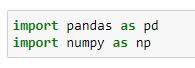
\includegraphics{Assets/Images/Pandas/import}
	\caption{Importing Pandas as pd}
	\label{fig:import}
\end{figure}

\noindent We would then load our dataset and import them as Pandas dataset.

\begin{figure}[ht]
	\centering
	\includegraphics[width=1.0\linewidth]{"Assets/Images/Pandas/read data"}
	\caption{Importing data}
	\label{fig:read-data}
\end{figure}

\noindent We can simply call the data by typing it's name (in this case \textit{drug}).
\begin{figure}[ht]
	\centering
	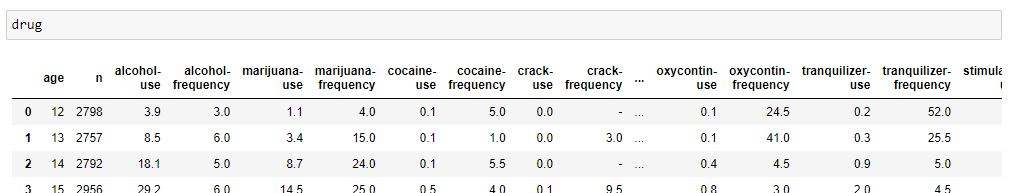
\includegraphics[width=1\linewidth]{Assets/Images/Pandas/drugs}
	\caption{Calling the data}
	\label{fig:drugs}
\end{figure}

\noindent If we only want to see the first few rows, we use the \textit{head} method. Which is 5 by default.

\begin{figure}[ht]
	\centering
	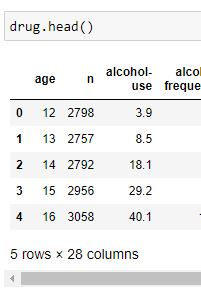
\includegraphics{Assets/Images/Pandas/head}
	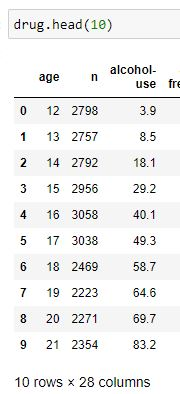
\includegraphics{Assets/Images/Pandas/head10}
	\caption{Using head method}
	\label{fig:head}
\end{figure}

\noindent Likewise, the \textit{tail} method for last few rows.

\begin{figure}[ht]
	\centering
	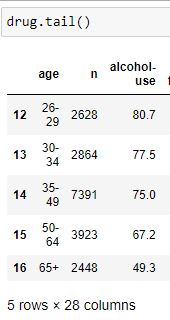
\includegraphics{Assets/Images/Pandas/tail}
	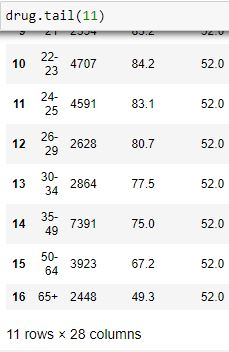
\includegraphics{Assets/Images/Pandas/tail11}
	\caption{Using tail method}
	\label{fig:tail}
\end{figure}

\newpage
\noindent The \textit{index} method is used to examine index which could be handy to detect duplicates

\begin{figure}[ht]
	\centering
	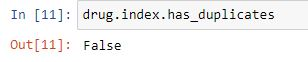
\includegraphics{Assets/Images/Pandas/index_duplicates}
	\caption{Using index method}
	\label{fig:index}
\end{figure}

\noindent We can use \textit{shape} method to examine the dimensions of our data.

\begin{figure}[ht]
	\centering
	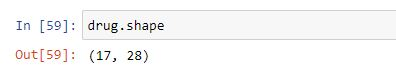
\includegraphics{Assets/Images/Pandas/shape}
	\caption{Using shape method}
	\label{fig:index}
\end{figure}
\chapter{Exponential and Logarithmic Functions}
\chapter{Limit and Differentiation}
\chapter{Linear Algebra, Vector and Matrices}
\chapter{Combinatorics and Probability}
\chapter{Little Gauss}
There is this story that is often told in mathematics classes. While the story itself is likely apocryphal, it likely have some pedagogical value. The story goes this way:

\vspace{5mm} %5mm vertical space

\noindent There was once a German school where a boy Carl Friedrich made mischief during mathematics lesson. Instead of corporal punishment that was common in that time, the teacher instead decided to give him mathematics assignment to keep him busy. He was asked to add up the numbers from one to a hundred. Most students would diligently start adding and be busy for a while. The young Carl Friedrich, on the other hand, answered after a few minutes. The teacher was surprised at the request to speak, since he had just kept the boy busy. He was all the more astonished when Carl Friedrich said that he had finished the task and was even able to say the correct result (5050).

\vspace{5mm} %5mm vertical space

\noindent{\large\textbf{How had he solved it?}}

\vspace{5mm} %5mm vertical space

\noindent How he did it so fast? Carl Friedrich discovered discovered the following - unfortunately I do not know what coincidence was behind it. He wrote the numbers down like this:

\begin{center}
\begin{tabular}{cccccc}
1   & 2  & 3  & $\mathellipsis$ & 99 & 100 \\
100 & 99 & 98 & $\mathellipsis$ & 2  & 1  
\end{tabular}
\end{center}

\noindent This still doesn't look interesting yet. He would then add up the numbers.

\begin{center}
\begin{tabular}{cccccc}
1   & 2  & 3  & $\mathellipsis$ & 99 & 100 \\
100 & 99 & 98 & $\mathellipsis$ & 2  & 1  \\
101 & 101 & 101 & $\mathellipsis$ & 101 & 101
\end{tabular}
\end{center}

\noindent Each of them have the sum 101. This looks rather promising. 

\vspace{5mm} %5mm vertical space 

\noindent To sum it up, we write down the numbers from one to one hundred twice, once in increasing order and once in decreasing order, we would then sum them up and we can clearly see that we obtain the sum of $100 \cdot 101$. But we are not finished yet because we counted each numbers twice so we still have to divide the results by two. Then, we would have the sum of numbers from one to a hundred. And that's exactly how Carl Friedrich proceeded. Do we know Carl Friedrich? Hopefully that's the case, because Carl Friedrich was none other than Carl Friedrich Gauss. One of the most important German mathematicians (if not the most important German mathematician).

\vspace{5mm} %5mm vertical space

\noindent{\large\textbf{Let us talk about the formula}}

\vspace{5mm} %5mm vertical space

\noindent Mathematicians love formulas or should I say the general solution of a problem. The sum of the first $n$ of natural numbers follows the formula:
\begin{equation}
\Sigma = \frac{n\cdot(n+1)}{2}
\end{equation}
\noindent This is not as complicated as it looks. We could for example count the sum of 1 to 150, then we set $n$ equals to 150.
\begin{equation}
\Sigma = \frac{150\cdot(150+1)}{2}= \frac{150\cdot(151)}{2}= \frac{22650}{2}=11325
\end{equation}
\noindent This formula is today is still affectionately referred as "Der Kleine Gauss", German for "Little Gauss". Anyone studying higher mathematics would have to prove the validity of the formula.
\chapter{How to prove it?}
\begin{figure}[htp]
	\centering
	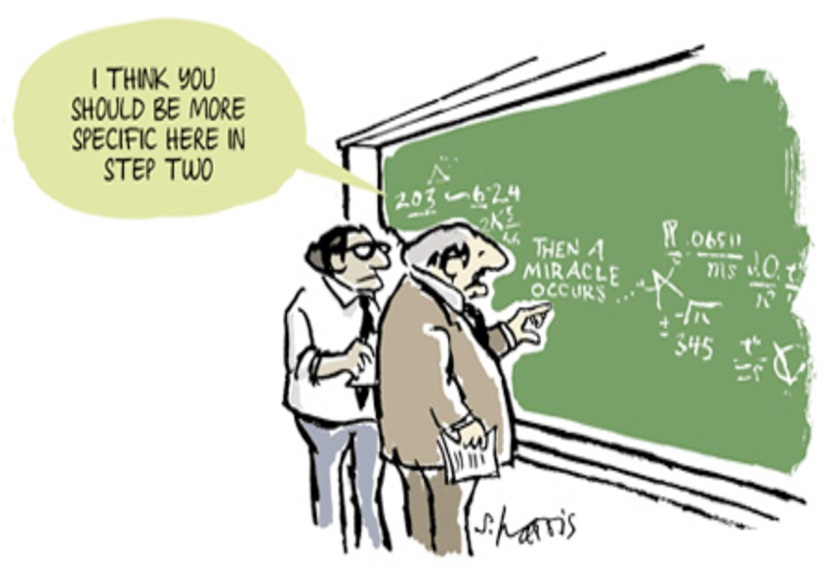
\includegraphics[width=\linewidth]{Assets/0_W-tEtGVYH9eM9HNx}
	\caption{}
	\label{fig:specific}
\end{figure}

\noindent One of the largest stumbling block in studying mathematics is learning how to prove theorems. In this post, I would share with you 3 of the most commonly used technique with at least one step by step example.
\newpage
\begin{enumerate}
\item \textbf{Direct proof}

\noindent Perhaps the most intuitive and straightforward way to write proofs. It goes by "\textit{If A, then B}" or  "\textit{A implies B}" or mathematically A $\Rightarrow$ B.

\begin{example}The sum of two even numbers is also even.
\begin{proof}
	Let $x$ and $y$ be even numbers. Since they are even, by definition they can be rewritten as $2n$ and $2m$ respectively. Thus, the sum $x+y = 2n+2m = 2(n+m)$, which is even number by definition.
\end{proof}
\end{example}
\begin{example}Third Binomial Formula
\begin{proof}
\begin{align}
(a-b)\cdot (a+b)&= a\cdot a+a\cdot b-b \cdot a-b \cdot b\\ 
			&= a^2+a \cdot b-b \cdot a-b^2\\ 
			&= a^2-b^2 
\end{align}
\end{proof}
\end{example}
\begin{example}Square of odd number is also odd
\begin{proof}
Let $x$ be odd numbers. Since it is odd, by definition it can be rewritten as $2n+1$. Thus the square product $x^2 = (2n+1)^2 = 4n^2+4n+1 = 2(2n^2+2n)+1$ which is an odd number by definition.
\end{proof}
\end{example}
\item \textbf{Indirect proof or proof by contradiction}

\noindent An elegant way to write a proof that might seem counter intuitive at first. It is also known as proof by contradiction and \textit{reductio ad impossibile}. It goes the following steps:
\begin{enumerate}
\item Assume the proposition to be proved is false
\item Then show that the assumption leads to mutually contradictory assertion
\item Since the assumption that the proposition is false proved contradictory, then the proposition must be true
\end{enumerate}
\newpage
\begin{example}Square root of two is irrational
\begin{proof}
Let there be $p$ such that $p^2=2$. 
If $p$ is rational, we could write $p = \frac{m}{n}$ where $m$ and $n$ are integers that are not both even. 
This is then implies that $m^2=2n^2$ and thus $m^2$ is even. If $m^2$ is even, $m$ must be even too. Because $m$ is even, $m^2$ is divisible by 4 which in turn implies that $n^2$ is even and therefore $n$ is even.
This contradicts with our earlier assumption that $m$ and $n$ are integers that are not both even and therefore, a rational $p$ could not exist.
\end{proof}
\end{example}
\begin{example}There exist no integers a and b for which 6a + 3b = 1
\begin{proof}
Let us first assume that such $a$ and $b$ exist.
Dividing by 3 gives us: $2a+b=\frac{1}{3}$
which is a contradiction since $2a+b$ is an integer but $\frac{1}{3}$ is not. Therefore there exist no such integers a and b
\end{proof}
\end{example}
\item \textbf{Mathematical Induction}

\noindent Mathematical induction is usually taught together with series and sequences. It is a powerful tool to prove series and sequences. It is split into two steps:
\begin{enumerate}
\item Initial case : prove that the statement holds for 0 and or 1
\item Induction step: show that the statement holds for every $n$, if it holds for $n$, then it also holds for $n+1$
\end{enumerate}

\begin{example}Little Gauss (Arithmetic progression)
\begin{equation}
\sum_{i=1}^n i= \frac{n\cdot(n+1)}{2}
\end{equation}
\begin{proof}
\textit{Initiation step} for n = 1:

\noindent For the left side:
\begin{equation}
	\sum_{i=1}^n i= 1
\end{equation}
And the right side:
\begin{equation}
	\frac{1\cdot(1+1)}{2}=1
\end{equation}
We obtain the same value from both sides, the equation holds for n = 1.

\textit{Induction step} from n to n+1:

\noindent For the left side:
\begin{equation}
	\sum_{i=1}^n i= 1
\end{equation}
And the right side:
\begin{equation}
	\frac{1\cdot(1+1)}{2}=1
\end{equation}
We obtain the same value from both sides, the equation holds for n = 1.
\end{proof}
\end{example}
\begin{example}Bernoulli's inequality
\begin{equation}
(1+x)^n \ge 1+nx
\end{equation}
\end{example}
\end{enumerate}
\chapter{misc unorganized stuffs}
use logic table to understand confusion matrix better

\backmatter
\bibliography{citation} 
\bibliographystyle{ieeetr}
% bibliography, glossary and index would go here.

\end{document}